\documentclass[a4paper,10pt]{article}
\usepackage{graphicx}
\usepackage[left=1in,right=1in,top=1in,bottom=1in]{geometry}
\usepackage{hyperref}
\usepackage{fancyhdr}

\pagestyle{fancy}
\lhead{\textbf{Daniel Velarde Kubber}}
\rhead{\textbf{Currículum Vitae}}
\cfoot{\thepage}

\begin{document}

% Agrega tu fotografía en la esquina superior derecha
\begin{minipage}[t]{0.7\textwidth}
  % Tu contenido existente va aquí
\end{minipage}
\hfill
\begin{minipage}[t]{0.3\textwidth}
  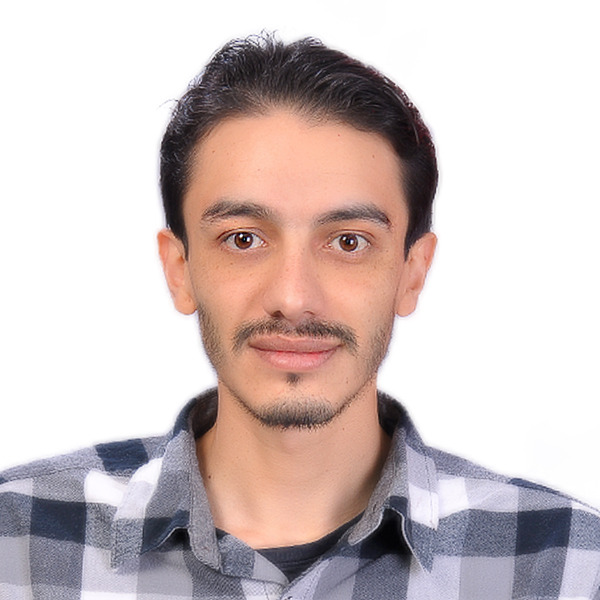
\includegraphics[width=2.5cm]{photocv.jpeg}
\end{minipage}

\begin{center}
\textbf{\LARGE Daniel Velarde Kubber}
\end{center}



\section*{Resumen Profesional}
Apasionado por los datos y la tecnología, soy un profesional orientado a resultados con antecedentes en Ingeniería Industrial y de Sistemas. Desde mis primeros días como administrador de bases de datos hasta mi papel como empresario y CEO en Hobbie 3D Print, he perfeccionado mis habilidades en la gestión de datos, el liderazgo estratégico y la competencia técnica.

Mi trayectoria profesional, que incluye experiencia práctica en la programación de impresoras 3D, administración de bases de datos y gestión de proyectos, refleja mi dedicación a aprovechar los datos para impulsar el éxito empresarial. Me impulsa el poder de la innovación y prospero en el desafío de fomentar el crecimiento.

Con un fuerte compromiso con la toma de decisiones basadas en datos, estoy emocionado por aplicar mi experiencia en nuevas oportunidades y contribuir a los campos de ingeniería de datos, análisis de datos y ciencia de datos.

\section*{Educación}
\begin{tabular}{p{3cm}p{12cm}}
    2012 & Ingeniero Industrial y de Sistemas, Universidad Privada Boliviana, Cochabamba - Bolivia \\
\end{tabular}



\section*{Licencias y Certificaciones}
\begin{description}
    \item[Certificado:] Introducción a la Ingeniería de Datos, Coursera, agosto de 2023
    \item[URL del Certificado:] \url{https://www.coursera.org/account/accomplishments/certificate/9S9DAUQLBP27}
\end{description}

\vspace{1pt} % Ajusta el valor para controlar la cantidad de espacio

\begin{description}
    \item[Certificado:] Introducción a las Bases de Datos Relacionales (RDBMS), Coursera, agosto de 2023
    \item[URL del Certificado:] \url{https://www.coursera.org/account/accomplishments/certificate/SG8MV2SLJXHC}
\end{description}

\vspace{1pt} % Ajusta el valor para controlar la cantidad de espacio

\begin{description}
    \item[Certificado:] Python para Ciencia de Datos, Inteligencia Artificial y Desarrollo, Coursera, agosto de 2023
    \item[URL del Certificado:] \url{https://www.coursera.org/account/accomplishments/certificate/X6P3RHPT255M}
\end{description}

\vspace{1pt} % Ajusta el valor para controlar la cantidad de espacio

\begin{description}
    \item[Certificado:] Proyecto Python para Ingeniería de Datos, Coursera, agosto de 2023
    \item[URL del Certificado:]\url{https://www.coursera.org/account/accomplishments/certificate/WEQ4BMAGTZZN}
\end{description}

\vspace{1pt} % Ajusta el valor para controlar la cantidad de espacio

\begin{description}
    \item[Certificado:] Introducción Práctica a los Comandos de Linux y Scripting de Shell, Coursera, septiembre de 2023
    \item[URL del Certificado:] \url{https://www.coursera.org/account/accomplishments/certificate/TN4F6WG8DWKB}
\end{description}

\vspace{1pt} % Ajusta el valor para controlar la cantidad de espacio

\begin{description}
    \item[Certificado:] Bases de Datos y SQL para Ciencia de Datos con Python, Coursera, septiembre de 2023
    \item[URL del Certificado:] \url{https://www.coursera.org/account/accomplishments/certificate/AZMNGATPHMYT}
\end{description}

\vspace{1pt} % Ajusta el valor para controlar la cantidad de espacio

\begin{description}
    \item[Certificado:] Administración de Bases de Datos Relacionales (DBA), Coursera, septiembre de 2023
    \item[URL del Certificado:] \url{https://www.coursera.org/account/accomplishments/certificate/EASM4DYAZY4L}
\end{description}

\vspace{1pt} % Ajusta el valor para controlar la cantidad de espacio

\begin{description}
    \item[Certificado:] ETL y Canalización de Datos con Shell, Airflow y Kafka, Coursera, septiembre de 2023
    \item[URL del Certificado:] \url{https://www.coursera.org/account/accomplishments/certificate/HGASHU2DN99L}
\end{description}
\vspace{1pt} % Ajusta el valor para controlar la cantidad de espacio
\begin{description}
  \item[Certificado:] Introducción a Big Data con Spark y Hadoop, Coursera, septiembre de 2023
  \item[URL del Certificado:] \url{https://www.coursera.org/account/accomplishments/certificate/JMZFZZETAGNK}
\end{description}
\vspace{1pt} % Ajusta el valor para controlar la cantidad de espacio
\begin{description}
  \item[Certificado:] Introducción a Bases de Datos NoSQL, Coursera, septiembre de 2023
  \item[URL del Certificado:] \url{https://www.coursera.org/account/accomplishments/certificate/UDUPYBEHNMW2}
\end{description}
\vspace{1pt} % Ajusta el valor para controlar la cantidad de espacio
\begin{description}
  \item[Certificado:] Empezando con Almacenamiento de Datos y Analítica de Inteligencia de Negocios, Coursera, septiembre de 2023
  \item[URL del Certificado:] \url{https://www.coursera.org/account/accomplishments/certificate/B88H4H6E8AFD}
\end{description}

\section*{Habilidades}
\begin{tabular}{p{4.5cm}p{4.5cm}p{4.5cm}}
    Bases de Datos & Arquitectura de Datos & Transferencia Electrónica de Fondos \\
    Seguridad de Bases de Datos & Diseño de Bases de Datos & Operaciones de Importación/Exportación \\
    Administración de Bases de Datos & RDBMS & Gestión de Inventarios \\
    Servidores de Bases de Datos & Canalización de Datos & Control de Inventarios \\
    SQL & Visualización de Datos & Contabilidad Básica \\
    IBM Db2 & Bokeh & Gestión de Proyectos \\
    MySQL & Matplotlib & Marketing Digital \\
    NoSQL & Pandas & Microsoft Office \\
    ETL (Extract, Load, Transform) & NumPy & Modelado 3D \\
    Jupyter Notebook & IBM Cloud & Impresión 3D \\
    Python & Linux & Desarrollo de Productos \\
    C++ & C\# & \\
    PostgreSQL & & \\
\end{tabular}


\section*{Intereses}
En mi tiempo libre, tengo pasión por la lectura de libros de fantasía, sumergiéndome en mundos épicos que recuerdan a "El Señor de los Anillos" y "World of Warcraft". También disfruto de los videojuegos, tanto como forma de entretenimiento como para relacionarme con mis hijos.

Soy un aprendiz ávido y encuentro alegría en la programación, explorando varios lenguajes de programación y, en un momento, incursionando en el desarrollo de juegos con Unity. Además, tengo un lado creativo que expreso a través de la pintura de miniaturas, un pasatiempo que me permite combinar mi amor por el arte y la artesanía.

\section*{Referencias Personales}
\renewcommand{\refname}{}

\begin{thebibliography}{}

\bibitem{hobbie3dprint} Hobbie 3D Print
  \begin{description}
    \item[Nombre:] Daniel Velarde Kubber
    \item[Email:] daniel.velarde.kubber@gmail.com
    \item[Teléfono:] +591 76778873
    \item[Facebook:] \url{https://www.facebook.com/Hobbie3DPrint/}
  \end{description}

\bibitem{velardeconstrucciones} Velarde Construcciones SRL
  \begin{description}
    \item[Nombre:] Ing. Carlos Estrada Roblin
    \item[Email:] cestradaroblin@gmail.com
    \item[Teléfono:] +591 77538902
  \end{description}

\bibitem{acerosarequipa} Aceros Arequipa
  \begin{description}
    \item[Nombre:] Ing. Daniel Fernando Balandra Mallma
    \item[Email:] daniel.balandra@repareq.com
    \item[Teléfono:] +591 77200296
  \end{description}

\end{thebibliography}
\end{document}

